\documentclass[10pt,twocolumn]{article}
% Shared two-column preamble for the three research papers.
% Use with: \documentclass[10pt,twocolumn]{article}
% Then in main.tex: % Shared two-column preamble for the three research papers.
% Use with: \documentclass[10pt,twocolumn]{article}
% Then in main.tex: % Shared two-column preamble for the three research papers.
% Use with: \documentclass[10pt,twocolumn]{article}
% Then in main.tex: \input{../../shared/latex/twocolumn_preamble.tex}

\usepackage[margin=0.75in]{geometry}
\usepackage[utf8]{inputenc}
\usepackage[T1]{fontenc}
\usepackage{lmodern}
\usepackage{microtype}
\usepackage{amsmath,amssymb,amsthm}
\usepackage{graphicx}
\usepackage{booktabs}
\usepackage{caption}
\usepackage{subcaption}
\usepackage{hyperref}
\usepackage{url}
\usepackage{xcolor}
\usepackage{algorithm}
\usepackage{algorithmic}
\usepackage{multirow}
\usepackage{titlesec}
\usepackage{authblk}

\hypersetup{colorlinks=true,linkcolor=blue!50!black,citecolor=blue!50!black,urlcolor=blue!50!black}

\titleformat{\section}{\normalfont\large\bfseries}{\thesection}{0.6em}{}
\titleformat{\subsection}{\normalfont\bfseries}{\thesubsection}{0.5em}{}

\captionsetup{font=small,labelfont=bf,skip=4pt}
\setlength{\columnsep}{0.25in}
\setlength{\parskip}{2pt}

\newtheorem{theorem}{Theorem}
\newtheorem{proposition}[theorem]{Proposition}
\newtheorem{definition}[theorem]{Definition}


\usepackage[margin=0.75in]{geometry}
\usepackage[utf8]{inputenc}
\usepackage[T1]{fontenc}
\usepackage{lmodern}
\usepackage{microtype}
\usepackage{amsmath,amssymb,amsthm}
\usepackage{graphicx}
\usepackage{booktabs}
\usepackage{caption}
\usepackage{subcaption}
\usepackage{hyperref}
\usepackage{url}
\usepackage{xcolor}
\usepackage{algorithm}
\usepackage{algorithmic}
\usepackage{multirow}
\usepackage{titlesec}
\usepackage{authblk}

\hypersetup{colorlinks=true,linkcolor=blue!50!black,citecolor=blue!50!black,urlcolor=blue!50!black}

\titleformat{\section}{\normalfont\large\bfseries}{\thesection}{0.6em}{}
\titleformat{\subsection}{\normalfont\bfseries}{\thesubsection}{0.5em}{}

\captionsetup{font=small,labelfont=bf,skip=4pt}
\setlength{\columnsep}{0.25in}
\setlength{\parskip}{2pt}

\newtheorem{theorem}{Theorem}
\newtheorem{proposition}[theorem]{Proposition}
\newtheorem{definition}[theorem]{Definition}


\usepackage[margin=0.75in]{geometry}
\usepackage[utf8]{inputenc}
\usepackage[T1]{fontenc}
\usepackage{lmodern}
\usepackage{microtype}
\usepackage{amsmath,amssymb,amsthm}
\usepackage{graphicx}
\usepackage{booktabs}
\usepackage{caption}
\usepackage{subcaption}
\usepackage{hyperref}
\usepackage{url}
\usepackage{xcolor}
\usepackage{algorithm}
\usepackage{algorithmic}
\usepackage{multirow}
\usepackage{titlesec}
\usepackage{authblk}

\hypersetup{colorlinks=true,linkcolor=blue!50!black,citecolor=blue!50!black,urlcolor=blue!50!black}

\titleformat{\section}{\normalfont\large\bfseries}{\thesection}{0.6em}{}
\titleformat{\subsection}{\normalfont\bfseries}{\thesubsection}{0.5em}{}

\captionsetup{font=small,labelfont=bf,skip=4pt}
\setlength{\columnsep}{0.25in}
\setlength{\parskip}{2pt}

\newtheorem{theorem}{Theorem}
\newtheorem{proposition}[theorem]{Proposition}
\newtheorem{definition}[theorem]{Definition}

\newcommand{\doadiffusesrpsnrZerortThree}{3.2}
\newcommand{\doadiffusesrpsnrZerortSix}{3.0}
\newcommand{\doadiffusesrpsnrOneZerortThree}{0.9}
\newcommand{\doadiffusesrpsnrOneZerortSix}{1.0}
\newcommand{\doadiffusesrpsnrTwoZerortThree}{0.9}
\newcommand{\doadiffusesrpsnrTwoZerortSix}{1.4}
\newcommand{\doadiffusesrpharmonicsnrZerortThree}{3.2}
\newcommand{\doadiffusesrpharmonicsnrZerortSix}{2.8}
\newcommand{\doadiffusesrpharmonicsnrOneZerortThree}{0.9}
\newcommand{\doadiffusesrpharmonicsnrOneZerortSix}{1.0}
\newcommand{\doadiffusesrpharmonicsnrTwoZerortThree}{1.0}
\newcommand{\doadiffusesrpharmonicsnrTwoZerortSix}{1.5}
\newcommand{\doadiffusesrpnonsubsnrZerortThree}{3.3}
\newcommand{\doadiffusesrpnonsubsnrZerortSix}{2.3}
\newcommand{\doadiffusesrpnonsubsnrOneZerortThree}{1.0}
\newcommand{\doadiffusesrpnonsubsnrOneZerortSix}{1.4}
\newcommand{\doadiffusesrpnonsubsnrTwoZerortThree}{0.9}
\newcommand{\doadiffusesrpnonsubsnrTwoZerortSix}{1.3}
\newcommand{\doadiffusesrpnosnrwsnrZerortThree}{19.4}
\newcommand{\doadiffusesrpnosnrwsnrZerortSix}{26.5}
\newcommand{\doadiffusesrpnosnrwsnrOneZerortThree}{1.4}
\newcommand{\doadiffusesrpnosnrwsnrOneZerortSix}{1.5}
\newcommand{\doadiffusesrpnosnrwsnrTwoZerortThree}{1.0}
\newcommand{\doadiffusesrpnosnrwsnrTwoZerortSix}{1.5}
\newcommand{\doadiffusesrpplainsnrZerortThree}{4.5}
\newcommand{\doadiffusesrpplainsnrZerortSix}{8.3}
\newcommand{\doadiffusesrpplainsnrOneZerortThree}{1.5}
\newcommand{\doadiffusesrpplainsnrOneZerortSix}{2.9}
\newcommand{\doadiffusesrpplainsnrTwoZerortThree}{0.9}
\newcommand{\doadiffusesrpplainsnrTwoZerortSix}{1.4}
\newcommand{\doadiffusegccsnrZerortThree}{21.7}
\newcommand{\doadiffusegccsnrZerortSix}{28.6}
\newcommand{\doadiffusegccsnrOneZerortThree}{1.5}
\newcommand{\doadiffusegccsnrOneZerortSix}{2.0}
\newcommand{\doadiffusegccsnrTwoZerortThree}{1.0}
\newcommand{\doadiffusegccsnrTwoZerortSix}{1.6}
\newcommand{\doafansrpsnrZerortThree}{4.2}
\newcommand{\doafansrpsnrZerortSix}{2.6}
\newcommand{\doafansrpsnrOneZerortThree}{1.3}
\newcommand{\doafansrpsnrOneZerortSix}{1.6}
\newcommand{\doafansrpsnrTwoZerortThree}{0.9}
\newcommand{\doafansrpsnrTwoZerortSix}{1.3}
\newcommand{\doafansrpharmonicsnrZerortThree}{4.0}
\newcommand{\doafansrpharmonicsnrZerortSix}{2.4}
\newcommand{\doafansrpharmonicsnrOneZerortThree}{1.3}
\newcommand{\doafansrpharmonicsnrOneZerortSix}{1.6}
\newcommand{\doafansrpharmonicsnrTwoZerortThree}{1.0}
\newcommand{\doafansrpharmonicsnrTwoZerortSix}{1.4}
\newcommand{\doafansrpnonsubsnrZerortThree}{7.8}
\newcommand{\doafansrpnonsubsnrZerortSix}{20.1}
\newcommand{\doafansrpnonsubsnrOneZerortThree}{3.0}
\newcommand{\doafansrpnonsubsnrOneZerortSix}{3.5}
\newcommand{\doafansrpnonsubsnrTwoZerortThree}{1.5}
\newcommand{\doafansrpnonsubsnrTwoZerortSix}{1.9}
\newcommand{\doafansrpnosnrwsnrZerortThree}{4.8}
\newcommand{\doafansrpnosnrwsnrZerortSix}{4.6}
\newcommand{\doafansrpnosnrwsnrOneZerortThree}{1.7}
\newcommand{\doafansrpnosnrwsnrOneZerortSix}{1.8}
\newcommand{\doafansrpnosnrwsnrTwoZerortThree}{0.9}
\newcommand{\doafansrpnosnrwsnrTwoZerortSix}{1.4}
\newcommand{\doafansrpplainsnrZerortThree}{68.6}
\newcommand{\doafansrpplainsnrZerortSix}{75.7}
\newcommand{\doafansrpplainsnrOneZerortThree}{5.3}
\newcommand{\doafansrpplainsnrOneZerortSix}{5.6}
\newcommand{\doafansrpplainsnrTwoZerortThree}{1.7}
\newcommand{\doafansrpplainsnrTwoZerortSix}{2.1}
\newcommand{\doafangccsnrZerortThree}{25.7}
\newcommand{\doafangccsnrZerortSix}{34.3}
\newcommand{\doafangccsnrOneZerortThree}{2.0}
\newcommand{\doafangccsnrOneZerortSix}{2.0}
\newcommand{\doafangccsnrTwoZerortThree}{1.0}
\newcommand{\doafangccsnrTwoZerortSix}{1.4}
\newcommand{\rhoCdrRoomMin}{-0.95}
\newcommand{\rhoCdrRoomMax}{-0.90}
\newcommand{\rhocdrdb}{-0.77}
\newcommand{\rholeveldb}{-0.61}
\newcommand{\rhosnrdb}{-0.48}
\newcommand{\rhotiltdb}{+0.13}
\newcommand{\distcvcdrdb}{0.44}
\newcommand{\distcvleveldb}{0.70}
\newcommand{\distcvsnrdb}{1.07}
\newcommand{\distcvtiltdb}{0.76}
\newcommand{\distcvall}{0.59}
\newcommand{\distcvcdrlevel}{0.45}
\newcommand{\distcvcdrlevelrtSixZero}{0.24}
\newcommand{\distcvcdrrtSixZero}{0.24}
\newcommand{\distxroomall}{0.51}
\newcommand{\distxroomcdrlevel}{0.55}
\newcommand{\distxroomcdrlevelrtSixZero}{0.33}
\newcommand{\distxroomcdrrtSixZero}{0.33}
\newcommand{\distPredictMean}{0.75}
\newcommand{\distPrior}{0.90}
\newcommand{\distN}{108}
\newcommand{\beamMvdrMean}{7.4}
\newcommand{\beamMvdrMin}{2.6}
\newcommand{\beamMvdrMax}{10.8}
\newcommand{\beamDsMean}{0.2}
\newcommand{\beamDoaErrMax}{9.6}
\newcommand{\demoAzMedErr}{1.0}
\newcommand{\demoAzPNinetyErr}{7.0}
\newcommand{\demoRangeMedErr}{0.18}
\newcommand{\hwAvailable}{no}


\title{Where Is the Speaker? Silence-Informed Localization, Distance Cues
and Selective Beamforming on a 4-Mic ReSpeaker}
\author[1]{Luis Benvenuto}
\affil[1]{Independent Research}
\date{October 4, 2026}

\begin{document}
\twocolumn[
\maketitle
\begin{@twocolumnfalse}
\begin{abstract}
\noindent Service robots often hear through a small circular microphone
array but use it as a single microphone. We study what the four raw
microphones of a ReSpeaker USB v2.0 (6.4\,cm aperture) can add to a
robot's speech pipeline: the talker's angle, the talker's distance, and
the suppression of sound from other directions before neural denoising.
The common thread is a \emph{silence model}: the pitch-based voice
activity detector the pipeline already runs splits the stream into voice
and silence, and the silence frames give the cross-spectra of everything
that is not the talker. In image-source simulations of a reverberant room
with a voiced talker, using that model twice in SRP-PHAT -- subtracting
the noise cross-spectra and weighting bins by speech presence -- reduces
the angle error at 0\,dB SNR with a directional fan from
\doafansrpplainsnrZerortThree/\doafansrpplainsnrZerortSix$^\circ$ (plain
SRP-PHAT, RT$_{60}$ 0.3/0.6\,s) to \doafansrpsnrZerortThree/\doafansrpsnrZerortSix$^\circ$, and a
streaming tracker follows a moving talker with a median error of
\demoAzMedErr$^\circ$. Distance cannot come from time differences on this
aperture; the coherent-to-diffuse ratio is the useful cue (Spearman
\rhocdrdb{} with log-distance across rooms), but it is room-relative:
cross-room distance error is \distxroomcdrlevel\,m with CDR and level and
\distxroomcdrrtSixZero\,m once the room's RT60 is given as a covariate,
against \distPredictMean\,m for predicting the mean. An MVDR beamformer
steered at the estimated talker, with its noise covariance learned while
the target is silent, improves output SINR against a competing talker by
\beamMvdrMean\,dB on average (\beamMvdrMin--\beamMvdrMax), while
delay-and-sum gains \beamDsMean\,dB. All results are simulation-only; the
code ships a live radar, recording and calibration tools for the hardware
evaluation, and a plan to integrate the method into a ROS~2 HRI pipeline.
\end{abstract}
\vspace{1em}
\end{@twocolumnfalse}
]

\section{Introduction}

Robots that take spoken commands in homes and competitions face the
cocktail-party problem with very little hardware. A common choice is the
ReSpeaker USB Mic Array v2.0: four omnidirectional microphones on a
32\,mm-radius circle with an on-chip DSP that outputs one processed channel
and a firmware direction-of-arrival (DOA) estimate. Our robot's speech
pipeline uses exactly that processed channel: it feeds a neural denoiser
(DeepFilterNet3 \cite{schroeter2023deepfilternet3}), then a voice activity
detector (VAD) built from an energy gate, an autocorrelation pitch test in
85--255\,Hz and an MFCC speaker lock, then speech recognition. Spatial
information is discarded, and the published firmware DOA is smoothed with
a linear average, which maps a talker crossing $0^\circ$ to $180^\circ$.

We ask what the raw microphones can add, in three steps a robot needs:
\emph{where} the talker is (angle), \emph{how far} (distance), and
\emph{attending} to them by suppressing other directions before the
denoiser. Our organising idea is that the VAD already provides the most
useful reference signal: frames without voice describe the room -- fans,
motors, diffuse noise -- and their cross-spectra can be used to clean the
localisation and to train the spatial filter.

Contributions: (i) a streaming localiser (pitch VAD $\to$ silence model
$\to$ SRP-PHAT $\to$ distance features $\to$ wrap-safe tracker) with an
ablation of each use of the silence model; (ii) an analysis of which
acoustic cues give distance on a 6.4\,cm array, showing that the
coherent-to-diffuse ratio works within a room and that a room covariate
(RT60) is what makes it transfer; (iii) a measurement of MVDR versus
delay-and-sum selectivity on this aperture with an estimated, not oracle,
steering direction; (iv) tools for the hardware study (live radar,
labelled recording, calibration) and an integration plan for a ROS~2
pipeline. All quantitative results here are from simulation; the hardware
evaluation is the next step and the paper says where we expect simulation
to be optimistic.

\section{Related work}

\paragraph{DOA with small arrays.} GCC-PHAT \cite{knapp1976gcc} and
steered-response power with PHAT weighting (SRP-PHAT)
\cite{dibiase2001srp} are the standard robust estimators under
reverberation; ODAS \cite{grondin2019odas} runs SRP-PHAT with tracking on
the same ReSpeaker and similar arrays for robots. Speech-presence or
SNR-dependent weighting of time--frequency bins is a known improvement for
GCC-type methods in noise; we evaluate it, and noise cross-spectrum
subtraction, as two uses of one silence model.

\paragraph{Distance estimation.} Source distance from a compact array
relies on the direct-to-reverberant ratio (DRR), level, or learned
features \cite{vesa2009binaural}. The coherent-to-diffuse ratio (CDR) is a
coherence-based DRR proxy with closed-form estimators
\cite{schwarz2015cdr}; it depends on the room's critical distance, which
scales with $\sqrt{V/\mathrm{RT}_{60}}$ \cite{kuttruff2016room}.

\paragraph{Spatial filtering before enhancement.} MVDR beamforming
\cite{capon1969mvdr} followed by single-channel enhancement is the classic
multichannel speech-enhancement chain; small-aperture arrays need
superdirective designs and are sensitive to steering errors. Neural
single-channel denoisers such as DeepFilterNet3
\cite{schroeter2023deepfilternet3} remove stationary and diffuse noise but
cannot separate two talkers by direction.

\paragraph{Simulation.} We use the image-source method
\cite{allen1979image} via pyroomacoustics \cite{scheibler2018pra}, and a
diffuse noise field with the exact spherical-isotropic coherence
\cite{habets2008diffuse}.

\section{Method}

\paragraph{Signal model.} Four microphones $p_m$ on a 32\,mm circle, 16\,kHz,
512-point Hann STFT, hop 256. A far-field source at azimuth $\theta$ gives
$X_m(f)=S(f)e^{-j2\pi f\tau_m(\theta)}$, $\tau_m=-p_m^\top u(\theta)/c$. The
largest inter-microphone delay is 0.19\,ms ($\approx$3 samples).

\paragraph{VAD and silence model.} Per frame, the mean of the four
channels over the last 1024 samples passes an energy gate and an
autocorrelation test: the normalised autocorrelation peak in the lag band
of 85--255\,Hz must exceed 0.6 (the robot pipeline's rule), which also
yields $F_0$. The gate is $\max(g_0, \phi\cdot 10^{6/20})$ where $\phi$
follows the RMS of non-speech frames (fast down, slow up), because the raw
microphones are not gain-controlled. Non-speech frames, after a 0.3\,s
hangover, update the noise cross-spectral matrix $\Phi_n$ (time constant
2\,s). Speech frames update $\Phi_x^{\text{fast}}$ (0.25\,s) and
$\Phi_x^{\text{slow}}$ (1\,s); both are reset when speech resumes after
0.6\,s of silence.

\paragraph{Angle.} SRP-PHAT on a $1^\circ$ grid in 200--3800\,Hz:
\[
P(\theta)\propto\sum_{i<j}\sum_f w_f\,\mathrm{Re}\Big\{\tfrac{R_{ij}(f)}{|R_{ij}(f)|}
e^{j2\pi f(\tau_i(\theta)-\tau_j(\theta))}\Big\},
\]
with $R=\Phi_x^{\text{fast}}-\Phi_n$ (noise subtraction) and
$w_f=\max(0,1-\mathrm{tr}\,\Phi_n/\mathrm{tr}\,\Phi_x)$ (speech-presence
weight). Optional: a Gaussian comb at multiples of $F_0$. The peak is
refined parabolically; confidence is the peak's height above the map
mean. Baseline: per-pair GCC-PHAT upsampled $16\times$ and a least-squares
fit of $u(\theta)$.

\paragraph{Distance.} From $\Phi_s=\Phi_x^{\text{slow}}-\Phi_n$: (a) CDR
with the DOA-independent estimator of \cite{schwarz2015cdr} per pair,
using bins where the diffuse coherence $\mathrm{sinc}(2\pi fd/c)<0.7$ in
0.4--7\,kHz, median over bins and over the six pairs; (b) speech level
(dBFS); (c) SNR over $\Phi_n$; (d) spectral tilt. A ridge regression maps
standardised features to $\log r$; RT$_{60}$ can be appended as a room
covariate (the ReSpeaker firmware reports an estimate).

\paragraph{Tracking.} An alpha-beta filter on the circle (residuals
wrapped to $[-180^\circ,180^\circ)$) and an EMA of $\log r$; measurements
below a confidence threshold are ignored, and tracks expire after 3\,s.

\paragraph{Selective filtering.} MVDR
$w=(\Phi_n+\delta I)^{-1}a/(a^H(\Phi_n+\delta I)^{-1}a)$ steered at the
estimated azimuth, $\delta$ = 1\% of per-bin power, against delay-and-sum
$w=a/4$. In the beamforming experiment the target's azimuth is estimated
by SRP-PHAT on the difference between cross-spectra after and before the
target's onset, and $\Phi_n$ is the pre-onset covariance (interferer plus
noise).

\paragraph{Simulation.} A shoebox room (8$\times$7$\times$3\,m,
image-source order $\le$25, Sabine absorption for the target RT$_{60}$),
array at 1.1\,m height placed off-centre, mouth at 1.5\,m. The talker is
a synthetic voiced signal (random $F_0$ in 100--220\,Hz, vowel formants,
syllabic envelope, pauses), $-30$\,dBFS at 1\,m with $\pm$4\,dB effort
jitter in the distance sweep. Noise: spherically diffuse pink noise
\cite{habets2008diffuse} plus mic self-noise, optionally a directional
pink ``fan'' at $200^\circ$, 2\,m. Sweeps are listed in
Table~\ref{tab:setup}.

\begin{table}[t]
\centering\small
\begin{tabular}{@{}ll@{}}
\toprule
DOA & 8 angles $\times$ SNR \{0,10,20\} $\times$ RT$_{60}$ \{0.3,0.6\} $\times$ \{diffuse, fan\} \\
Distance & 6 distances 0.5--3\,m $\times$ 3 angles $\times$ RT$_{60}$ \{0.3,0.45,0.6\} $\times$ 2 \\
Beam & interferer at 45--180$^\circ$, SIR 0\,dB, RT$_{60}$ \{0.3,0.6\} \\
Demo & 7 positions, 0.5--3\,m, RT$_{60}$ 0.45, 17.5\,s \\
\bottomrule
\end{tabular}
\caption{Local simulation sweeps (\texttt{local\_small.yaml}).}
\label{tab:setup}
\end{table}

\section{Results}

\begin{figure*}[t]
\centering
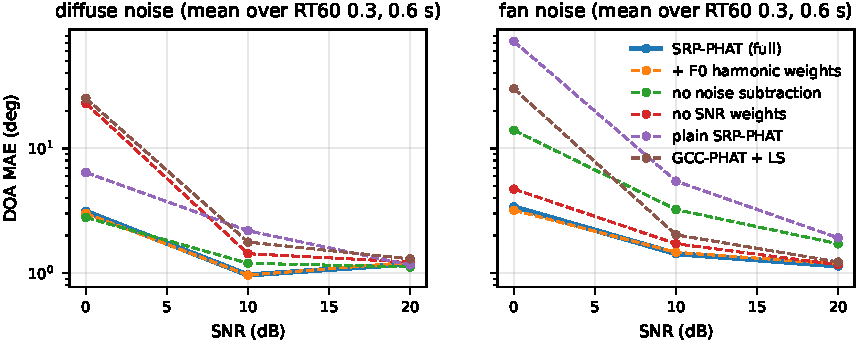
\includegraphics[width=\textwidth]{figures/doa_error.pdf}
\caption{DOA mean absolute error (log scale) versus SNR, averaged over
RT$_{60}$ 0.3 and 0.6\,s, talker at 1.5\,m. Removing either use of the
silence model hurts in one noise condition; removing both fails with a
directional noise source.}
\label{fig:doa}
\end{figure*}

\paragraph{Angle.} Figure~\ref{fig:doa}. At 20\,dB SNR all estimators are
within about $2^\circ$. At 0\,dB the two uses of the silence model matter in
different conditions. With diffuse noise, dropping the speech-presence
weights raises the error from \doadiffusesrpsnrZerortThree/\doadiffusesrpsnrZerortSix$^\circ$
(RT$_{60}$ 0.3/0.6\,s) to
\doadiffusesrpnosnrwsnrZerortThree/\doadiffusesrpnosnrwsnrZerortSix$^\circ$:
after subtraction, noise-only bins carry structured residue that PHAT
normalises to full weight. With the fan, dropping the subtraction raises it
from \doafansrpsnrZerortThree/\doafansrpsnrZerortSix$^\circ$ to
\doafansrpnonsubsnrZerortThree/\doafansrpnonsubsnrZerortSix$^\circ$, and
plain SRP-PHAT locks on the fan
(\doafansrpplainsnrZerortThree/\doafansrpplainsnrZerortSix$^\circ$).
GCC-PHAT with least squares reaches
\doadiffusegccsnrZerortThree--\doafangccsnrZerortSix$^\circ$ at 0\,dB. The
$F_0$-harmonic comb changes nothing measurable on our synthetic talker,
whose spectrum is already purely harmonic.

\begin{figure}[t]
\centering
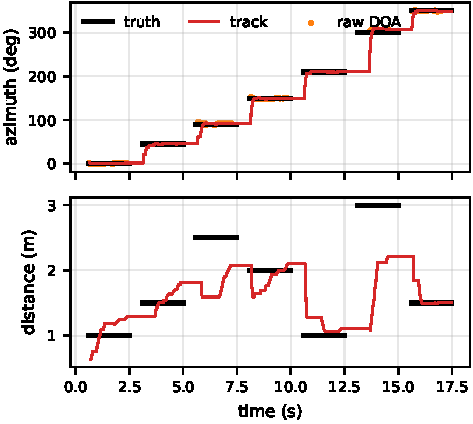
\includegraphics[width=\linewidth]{figures/radar_demo_track.pdf}
\caption{Streaming estimates for a talker moving through 7 positions
(black: truth). Top: azimuth. Bottom: distance.}
\label{fig:demo}
\end{figure}

\paragraph{Tracking a moving talker.} Figure~\ref{fig:demo}: after
0.5\,s of settling per position, the tracked azimuth has a median error of
\demoAzMedErr$^\circ$ (90th percentile \demoAzPNinetyErr$^\circ$). The
distance track (model trained in the same room) has a median error of
\demoRangeMedErr\,m and under-estimates the 3\,m position.

\begin{figure*}[t]
\centering
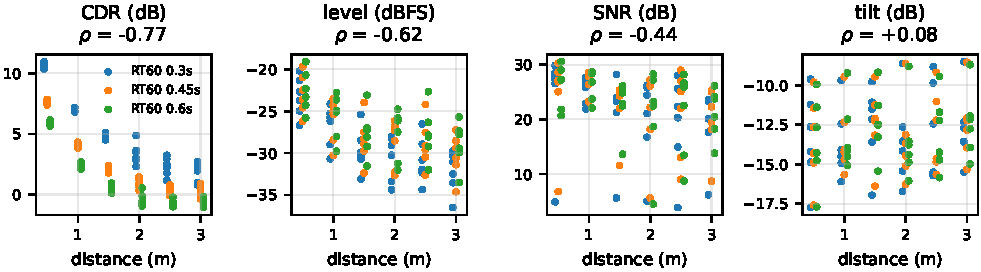
\includegraphics[width=\textwidth]{figures/distance_features.pdf}
\caption{Distance features versus true distance (\distN{} clips), coloured
by RT$_{60}$; $\rho$ is Spearman's correlation with $\log r$ over all
rooms. CDR is monotone within each room but offset between rooms.}
\label{fig:distfeat}
\end{figure*}

\begin{figure}[t]
\centering
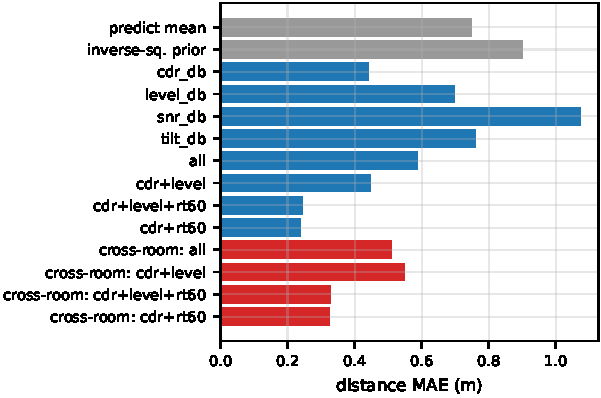
\includegraphics[width=\linewidth]{figures/distance_cv.pdf}
\caption{Distance MAE. Blue: leave-one-angle-out; red: leave-one-RT$_{60}$-out.}
\label{fig:distcv}
\end{figure}

\paragraph{Distance.} Figure~\ref{fig:distfeat}: the CDR is the strongest
cue ($\rho=\rhocdrdb$ pooled, \rhoCdrRoomMax{} to \rhoCdrRoomMin{} within a room). Level
($\rho=\rholeveldb$) suffers from the $\pm$4\,dB vocal-effort jitter, SNR
($\rhosnrdb$) from how much speech leaks into the noise estimate, and tilt
($\rhotiltdb$) carries little information. Figure~\ref{fig:distcv}: across
angles, CDR alone gives \distcvcdrdb\,m MAE and CDR + level
\distcvcdrlevel\,m, against \distPredictMean\,m for predicting the mean and
\distPrior\,m for an inverse-square law on level. Adding the room's
RT$_{60}$ gives \distcvcdrrtSixZero\,m, and across rooms (leave one
RT$_{60}$ out) \distxroomcdrrtSixZero\,m versus \distxroomcdrlevel\,m
without it.

\begin{figure}[t]
\centering
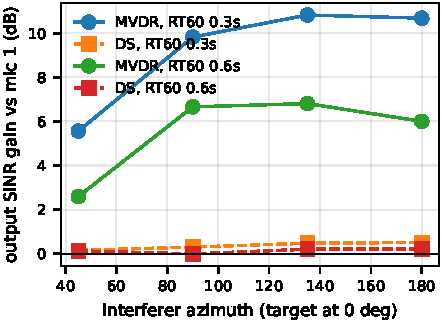
\includegraphics[width=\linewidth]{figures/beamform_gain.pdf}
\caption{Output SINR gain over microphone 1 against a competing talker
(target at $0^\circ$, both at 1.2\,m, SIR 0\,dB), with steering from the
estimated DOA.}
\label{fig:beam}
\end{figure}

\paragraph{Selective cancellation.} Figure~\ref{fig:beam}: MVDR gains
\beamMvdrMin--\beamMvdrMax\,dB (mean \beamMvdrMean\,dB), less in the more
reverberant room and at $45^\circ$ separation, where the estimated target
DOA was also furthest off (\beamDoaErrMax$^\circ$). Delay-and-sum gains
\beamDsMean\,dB: at 1\,kHz the array spans 0.19 wavelengths, so only
superdirective weights give selectivity.

\section{Discussion}

\paragraph{The silence model is the method.} The estimators are textbook.
What made them work on this array was getting ``noise'' right: which bins
contain it, which frames it can be learned from (a fixed energy gate tuned
for the processed channel missed a talker at 3\,m entirely), and when old
statistics stop describing the scene (a talker who moved between
utterances). The robot pipeline's VAD already provides the voice/silence
split, so these gains come without new sensing.

\paragraph{Distance is a room-calibrated quantity.} A 6.4\,cm array has no
geometric range resolution; the CDR measures distance relative to the
room's critical distance. This predicts, and the cross-room experiment
confirms, that a room descriptor is needed. The ReSpeaker firmware's RT$_{60}$
estimate is a candidate; its accuracy is untested. Without it, a short
calibration per room (a few labelled utterances) or coarse
near/mid/far buckets are the realistic outputs.

\paragraph{Where simulation is optimistic.} The synthetic talker is more
periodic and spectrally simpler than speech, which helps both the VAD and
PHAT; the shoebox image-source model has specular reflections and no
furniture, scattering or robot body; the diffuse field is ideal; and the
microphones are perfectly matched and positioned. Real recordings will
also reveal the mapping between raw channels, our azimuth convention and
the firmware's. We expect larger angle errors at low SNR and a weaker
within-room CDR correlation on hardware.

\paragraph{Limitations.} Small sweeps (8 clips per DOA cell, 108 distance
clips, 8 beamforming scenes) without confidence intervals; a larger
configuration is provided. One interferer, equal levels; no moving
interferer; no own-voice (TTS) handling; MVDR's noise covariance in the
beamforming experiment comes from a clean pre-onset segment.

\section{Conclusion}

On a four-microphone, 6.4\,cm array, the voice/silence split a robot's
speech pipeline already computes is enough to turn the raw channels into
a usable sense of where the talker is: a few degrees of angle error at
0\,dB SNR when the silence frames are used both to subtract noise and to
weight frequency bins, distance within about a third of a metre once the
room's reverberation is known, and several dB of suppression of a
competing talker with an MVDR filter steered at the estimate. Next steps
are the hardware evaluation with labelled recordings (including the
firmware DOA as a baseline and its RT$_{60}$ estimate as the room
covariate), and integrating the localiser and spatial filter as ROS~2
nodes ahead of the existing DeepFilterNet3 denoiser, evaluated by speech
recognition accuracy with two simultaneous talkers.

\paragraph{Reproducibility.} \texttt{make all} in
\texttt{projects/15\_spatial\_audio\_attention} regenerates every number
and figure from the simulation in about three minutes on a laptop CPU;
\texttt{make live}, \texttt{make record} and \texttt{make calibrate} run
the hardware study.


\FloatBarrier
\bibliographystyle{plain}
\bibliography{references}

\end{document}
